\documentclass[12pt,a4paper]{article}
\usepackage[utf8]{inputenc}
\usepackage{amsmath}
\usepackage{amsfonts}
\usepackage{amssymb}
\usepackage{graphicx}
\usepackage{subcaption}
\usepackage[top=2in, bottom=1.5in, left=1in, right=1in]{geometry}
\usepackage{fancyhdr}
\pagestyle{fancy}
\fancyhf{}
\rhead{Hunter King B00528551\\Alex Rudiuk \textbf{B00...}}
\author{Hunter King and Alex Rudiuk}
\title{CSCI 6505 Assignment $\#$7}
\begin{document}
\section*{CSCI 6505 Assignment $\#$7}
\subsection*{Intro}
This assignment explores and compares reinforcement learning through the use of a static \textbf{look-up table??} and a function approximator as a means to learn to play tic-tac-toe and ``four in a row". Initially the system was trained against itself using the Q-learning algorithm as a means of training. Once the system was trained, a second system composed of a function approximator that used a sigmoidal multilayer perceptron was also trained. This second system used the same Q-learning algorithm to update the weights of the function approximator, but also used a back propagation method to update the weights once each game was completed.\\
It should be noted to give context to the results that if an individual knows how to play tic-tac-toe well they should never lose due to a rather limited number of ways to play. This then extends such that if two players who both know how to play play against each other, the result will always be a tie. This also extends to ``four-in-a-row"
\subsection*{Methods}
The first method used for tic-tac-toe was the Q-learning algorithm utilizing a lookup table. The lookup table stores the value of every potential board state. These values were stored in a 9 dimensional array such that the system can quickly point to an index and retrieve the corresponding value of the state instead of searching through a list for the state in question. though this method requires a significant amount of memory, it also allows for a significant increase in training (and testing) speed. The lookup table was initialized with random values ranging from $[-0.5 \rightarrow 0.5]$. Once the system was initialized, it was trained by playing against itself for 3 million games, updating the table through the Q-learning method (equation \ref{eq:q-learning}). 
\begin{equation}
{Q(s,a)} \leftarrow {Q(s,a) + \mu(r + \gamma max_{a'}Q(s',a')-Q(s,a))}
\label{eq:q-learning}
\end{equation}
The results of the training are shown in figure \ref{fig:training}
\begin{figure}[h]
\centering
\includegraphics[width=0.8\textwidth]{figures/train01epsilon.png}
\caption{Average results over training period. Bins are 10000 games}
\label{fig:training}
\end{figure}
The plot shows an average of $\sim$32\% wins. Meaning that 32/100 games end in not a tie. This imperfect result is due to our $\epsilon$ (random action selection) which we set to 0.1. Figure BB show the results of the same trained system, but with $\epsilon$=0, playing against a version of itself with $\epsilon$=0.1.
\begin{figure}[h]
\centering
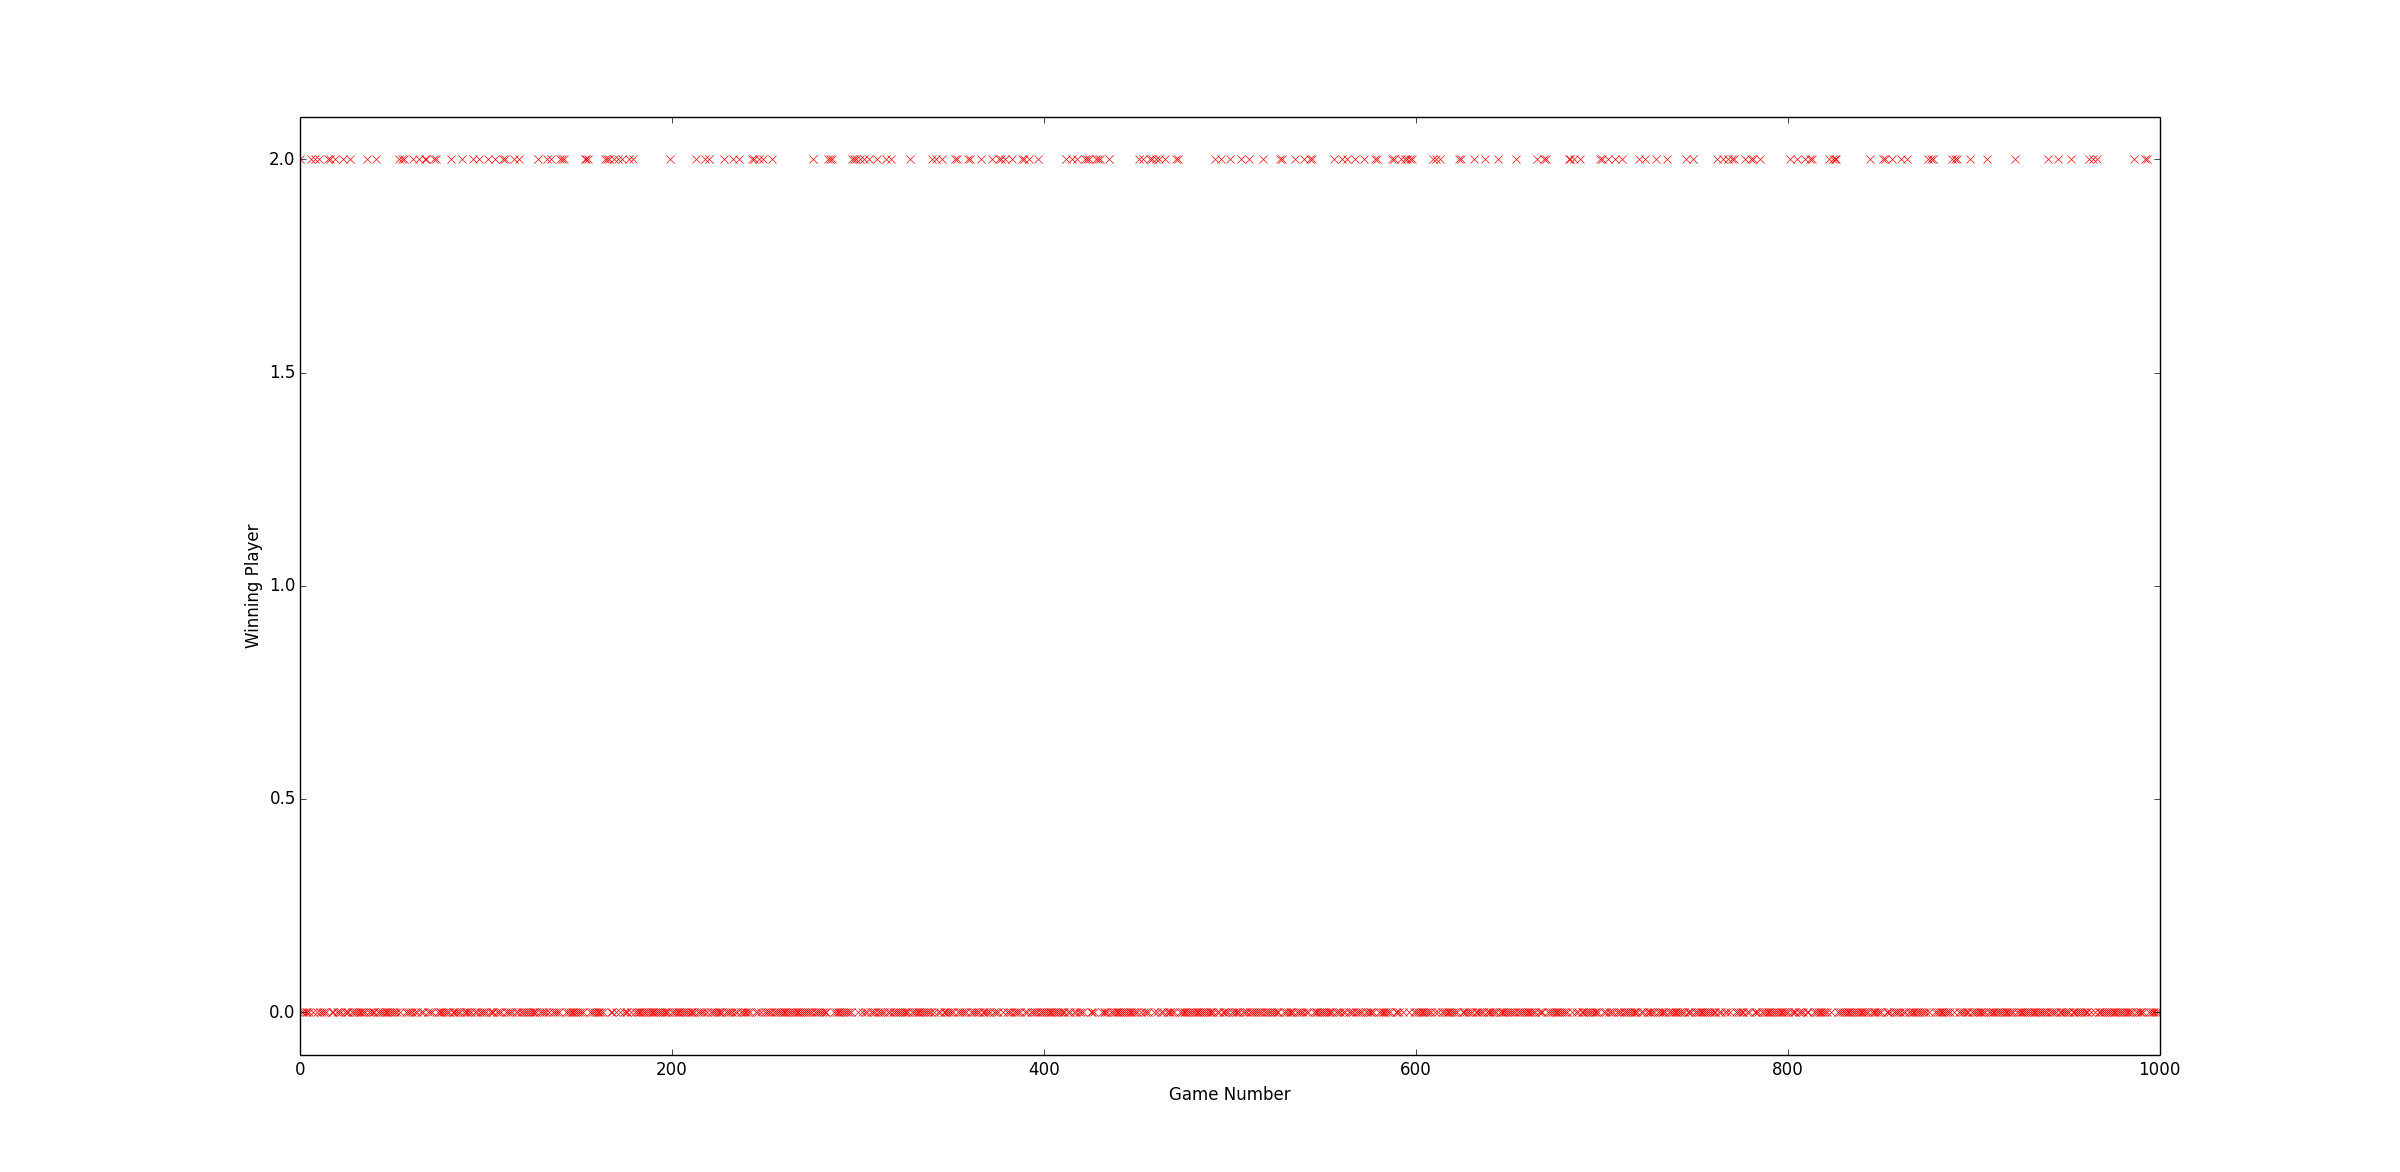
\includegraphics[width=0.8\textwidth]{figures/Optimalstateresults.png}
\caption{Results of trained system playing against itself (player $\epsilon$=0, opponent $\epsilon$=0.1)}
\label{fig:training}
\end{figure}
The output is 2.0 whenever the player with $\epsilon$=0 wins, and is 1.0 when the player with $\epsilon$=0.1 wins. This proves that our system has learned to properly play the game as both players mostly tie, however due to the 10\% chance of a random move by the opponent, the player sometimes wins (though never loses).
\subsection*{Conclusions}

\end{document}